\chapter{Real World Adoption \& Use-Cases}
\label{chap:real_world}

In recent years, the adoption of Rust has grown substantially within large-scale software projects and technology companies. This trend is evident both in the complete rewriting of existing infrastructures originally implemented in languages such as C++ and in the development of new components in Rust that interoperate with legacy C++ codebases. Notably, C++—along with its predecessor, C—has served as an industry stalwart since the 1990s.

\paragraph{}

\begin{figure}[H]
    \centering
    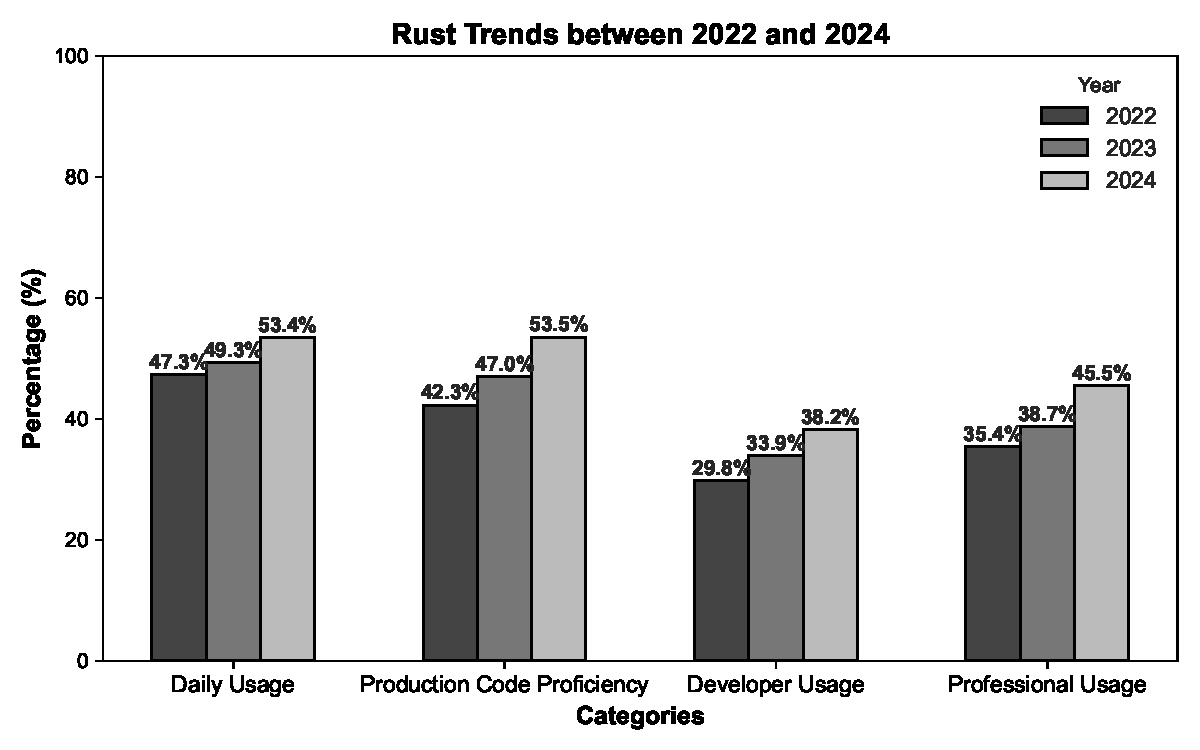
\includegraphics[width=\linewidth]{images/grouped_bar_chart.pdf}
    \caption{Adoption Trends and Proficiency in Rust according to 2024 State of Rust Survey \cite[]{2024StateRust}.}
    \label{fig:bargraph}
\end{figure}

According to the 2024 State of Rust survey \cite[]{2024StateRust}, 63.7\% of respondents indicated that they no longer use Rust but would like to in the future if the opportunity arises. Meanwhile, 36.0\% of respondents cited external factors, such as changing goals and requirements in their professional use of Rust, as the reason for no longer using it. This marks a decrease from 45.7\% in 2023, possibly indicating that Rust is becoming more integrated into professional development settings.

This trend is further supported by the continuous increase in daily or near-daily Rust usage, which grew from 47.3\% in 2022 to 49.3\% in 2023 and 53.4\% in 2024. Similarly, the percentage of participants who claim proficiency in writing production-ready Rust code has risen from 42.3\% in 2022 to 47.0\% in 2023, reaching 53.5\% in 2024. This suggests a growing number of proficient Rust developers producing usable code.

The proportion of developers using Rust for the majority of their coding tasks has increased from 29.8\% in 2022 to 33.9\% in 2023 and 38.2\% in 2024, indicating a rising adoption of Rust in professional settings. This is further reinforced by the increase in organizations making non-trivial use of Rust, from 35.4\% in 2022 to 38.7\% in 2023 and 45.5\% in 2024 \cite[]{2024StateRust}.

\paragraph{}

Microsoft exemplifies a leading proponent of this shift. As one of the organizations with the largest codebases in C and C++ globally \cite[]{2022ReviewAdoption}, Microsoft initiated a significant transition in 2020 by rewriting its implementation of DWriteCore. This effort has yielded a hybrid codebase consisting of 152,000 lines of Rust and 96,000 lines of C++ code. Additionally, the Windows Win32 GDI is currently being ported to Rust, with 36,000 lines of Rust code integrated so far \cite[]{claburnMicrosoftRewritingCore}.

\paragraph{}

A community fork of the Linux kernel, known as Rust for Linux (RFL), was created in 2020 with the goal of leveraging Rust's memory safety features to reduce bugs in kernel driver development. The first Rust-based drivers were introduced in Linux kernel version 6.8 \cite[]{EmpiricalStudyRustforLinux2024}.

In 1992, the possibility of incorporating C++ into the Linux kernel was briefly considered but ultimately rejected, with Linus Torvalds expressing strong opinions against both the C++ language and its compiler \cite[]{LinusTorvalds}.

A study by H. Li et al. \cite[]{EmpiricalStudyRustforLinux2024} analyzed the progress of RFL, focusing on security aspects, particularly bug mitigation and the use of unsafe Rust. The authors argue that Rust’s safety mechanisms help developers fix existing kernel bugs while significantly reducing the likelihood of introducing new memory-related issues. This, in turn, reduces the cognitive load required to ensure kernel safety.

They acknowledge that while the use of unsafe Rust is unavoidable, vulnerabilities are not. Additionally, Rust's strict ownership rules necessitate the use of unsafe Rust in some cases to streamline review cycles. However, they also highlight that some bugs become more obscure, requiring expertise in both Rust and kernel development to debug effectively. For example, a use-after-free bug in C may transform into a mapping bug in Rust, which is not detected by the Rust compiler.

Finally, their study found that Rust’s safety features lead to a significant increase in binary size, though performance remains comparable to C implementations in some cases \cite[]{EmpiricalStudyRustforLinux2024}.